\documentclass{sig-alternate}
%\documentclass[a4paper,10pt]{article}
\usepackage[utf8]{inputenc}
%El template pincha con spanish babel
%\usepackage[spanish]{babel}
\usepackage{amsmath, amssymb, amsfonts}
\usepackage{graphicx}
\usepackage{fancybox}
\usepackage[table]{xcolor}
\usepackage{soul}

\newtheorem{theorem}{Teorema}

\title{TITULAME} 

\numberofauthors{4}
\author{
\alignauthor
Pose, Alberto Miguel\\
       \affaddr{Instituto Tecnol\'ogico de Buenos Aires}\\
       \affaddr{Buenos Aires, Argentina}\\
       \email{apose@alu.itba.edu.ar}
\alignauthor
Catalano, Juan Ignacio\\
       \affaddr{Instituto Tecnol\'ogico de Buenos Aires}\\
       \affaddr{Buenos Aires, Argentina}\\
       \email{jcatalan@alu.itba.edu.ar}
\and
\alignauthor 
Palombo, Mart\'in\\
       \affaddr{Instituto Tecnol\'ogico de Buenos Aires}\\
       \affaddr{Buenos Aires, Argentina}\\
       \email{mpalombo@alu.itba.edu.ar}
\alignauthor 
V\'azquez, Santiago Jos\'e\\
       \affaddr{Instituto Tecnol\'ogico de Buenos Aires}\\
       \affaddr{Buenos Aires, Argentina}\\
       \email{savazque@alu.itba.edu.ar}
}

\date{}

\begin{document}

\maketitle

\begin{abstract}
Se estudia el generador de n\'umeros pseudaleatorios de L'Ecuyer.
Se lo somete a los tests Chi Cuadrado y Kolmogorov-Smirnov.
Luego, se lo utiliza para estimar el tiempo medio de vuelo de
la nave USS Enterprise mediante simulaci\'on de Montecarlo.
\end{abstract} 

\newpage

\section{Introducci\'on}
Los generadores lineales congruentes(GLC) son uno de los algoritmos
para generar n\'umeros pseudoaleatorios m\'as estudiados.
Estos generadores son definidos por la relaci\'on de recurrencia
\eqref{eq:lcg} donde $X_n$ es la secuencia de n\'umeros pseudoaleatorios y
 $m > 0$ es el m\'odulo, $a$ ($ 0 < a < m$) el multiplicador, $c$ ($0 \leq c < m$)
el incremento y $X_0$ la semilla o valor inicial. \\

Es deseable que los generadores de n\'umeros pseudoaleatorios cumplan
con ciertas propiedades. Las m\'as importantes son las de uniformidad
e independencia. \\

En la secci\'on \ref{sec:goingdown} se aplican tests estad\'isticos para
verificar ambas propiedades sobre el generador de L'Ecuyer. En la secci\'on
\ref{sec:triangle} se muestra como se pueden utilizar los GLC para obtener
una realizaci\'on de una variable aleatoria de una distribuci\'on cualquiera.
En la secci\'on \ref{sec:buzzlightyear} se utiliza un GLC para estimar el
tiempo medio de vuelo de la nave USS Enterprise.

\begin{equation}
\label{eq:lcg}
X_{n+1} = (aX_{n}+c) mod m
\end{equation}

\section{Atacando a L'Ecuyer}
\label{sec:goingdown}

\subsection{Generador de L'Ecuyer}
\label{sec:ecuyer_intro}
El generador sugerido por L'Ecuyer (1998) combina dos LCG\'s seg\'un el
siguiente algoritmo:
\par PASO 1 seleccionar una semilla $X_{1,0}$ en el rango $[1,2147483562]$ para el 
LCG1, y $X_{2,0}$ en el rango $[1,2147483398]$ para el LCG2.
\par PASO 2 evaluar cada generador individual

\begin{equation}
	X_{1,n+1} = 40014 X_{1,n} \quad mod \quad 2147483563
\end{equation}

\begin{equation}
	X_{2,n+1} = 40692 X_{2,n} \quad mod \quad 2147483399
\end{equation}


\par PASO 3 Computar

\begin{equation}
	X_{n+1} = (X_{1,n+1} - X_{2,n+1} ) \quad mod \quad 2147483562
\end{equation}

\par PASO 4 Computar

\begin{equation}
	U_{n+1} =
	\begin{cases}
		\frac{X_{n+1}}{2147483563}, X_{n+1} > 0 \\
		\frac{2147483562}{2147483563}, X_{n+1} = 0 \\
	\end{cases}
\end{equation}

\par PASO 5 Hacer $n = n + 1$ e ir al PASO 2.

Se realiza un an\'alisis del generador de L'Ecuyer mediante los tests
Chi cuadrado(para analizar uniformidad) y Kolmogorov-Smirnov
(para analizar independecia).
Se hace una realizaci\'on de $10000$ muestras del generador de L'Ecuyer y se realian dichos tests.
Cabe destacar que para la realizaci\'on del generador de L'Ecuyer se utilizan las semillas 1 y 1 y
se agrupa dicha realizaci\'on en $10$ intervalos de clase. Los resultados de dicha realizaci\'on 
se observan en la figura \ref{fig:histograma_ecuyer}

\begin{figure}[ht]
\label{fig:histograma_ecuyer}
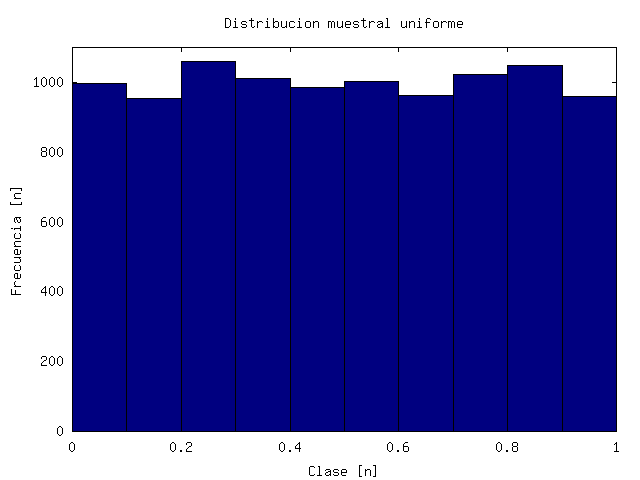
\includegraphics[width=8cm]{histograma_ecuyer}
\caption{Histograma de los 1000 n\'umeros agrupados en 10 intervalos de clase}
\end{figure}

\subsection{Test Chi Cuadrado}
\label{sec:chi}
Se aplica el test de Chi Cuadrado y se obtiene el estad\'istico $\chi_{0}^{2}=0.010003$.
Entonces, para $9$ grados de libertad y una significaci\'on de $\alpha=0.05$ se obtiene
el valor cr\'itico $\chi_{9,0.05}^{2}=16.92$.
Como $\chi_{0}^{2}=0.010003 < \chi_{9,0.05}^{2}=16.92$ se acepta la hip\'otesis $H_{0}$
de que la muestra provenga de una distribuci\'on uniforme.

\subsection{Test Kolmogorov-Smirnov}
\label{sec:kolmogorov}
Se aplica el test de Kolmogorov-Smirnov y se obtiene $D=0.99980$.
Para un nivel de significaci\'on $\alpha=0.05$ y $10$ intervalos de clase
se obtiene $D_{0.05}=0.410$. Entonces como $D > D_{\alpha}$
se acepta la hip\'otesis $H_{0}$ de que la muestra
provenga de una distribuci\'on uniforme.

\subsection{L'Ecuyer al desnudo}
Aunque el generador haya pasado los tests observados en las secciones \ref{sec:chi} y \ref{sec:kolmogorov}
es necesario ver como estan distribuidos los n\'umeros generados en el espacio. En todo GLC,
los n\'umeros generados yacen sobre hiperplanos (rectas en 2D, planos en 3D) bien definidos. Esto
sucede dado a la correlaci\'on entre los valores sucesivos del generador.
Sin embargo, si se posee un buen GLC, dichos hiperplanos son casi irreconocibles. Es por esto,
que se presenta la gr\'afica \ref{fig:ecuyer_2D} para observar lo que sucede en 2D.
Se puede observar que la gr\'afica se asemeja a una nube de puntos sobre la cual es
pr\'acticamente imposible distinguir recta alguna. \\


\begin{figure}[ht]
\label{fig:ecuyer_2D}
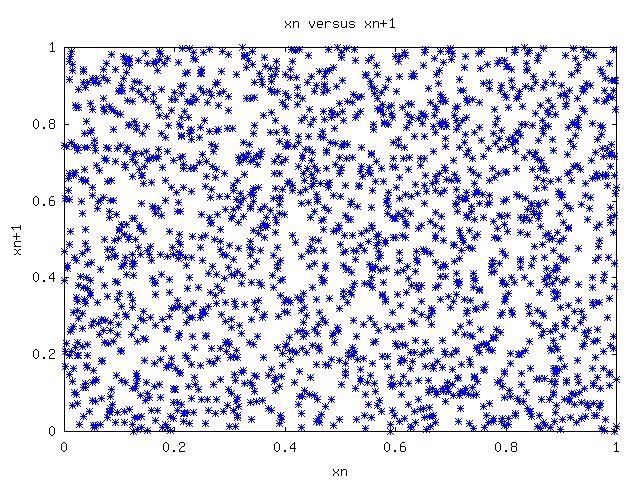
\includegraphics[width=8cm]{ecuyer2D}
\caption{Gr\'afica de $x_{n}$ versus $x_{n+1}$}
\end{figure}

Se repite el an\'alisis para 3D pero se toma el cuidado especial de genrar tres gr\'aficos rotados
para analizar lo que sucede en cada reg\'on. De este an\'alisis se obtienen las gr\'aficas
\ref{fig:ecuyer_3D_1}, \ref{fig:ecuyer_3D_2} y \ref{fig:ecuyer_3D_3}. Se puede observar
tambi\'en en este caso que no puede visualizarse ning\'un plano sobre la nube de puntos. \\

\begin{figure}[ht]
\label{fig:ecuyer_3D_1}
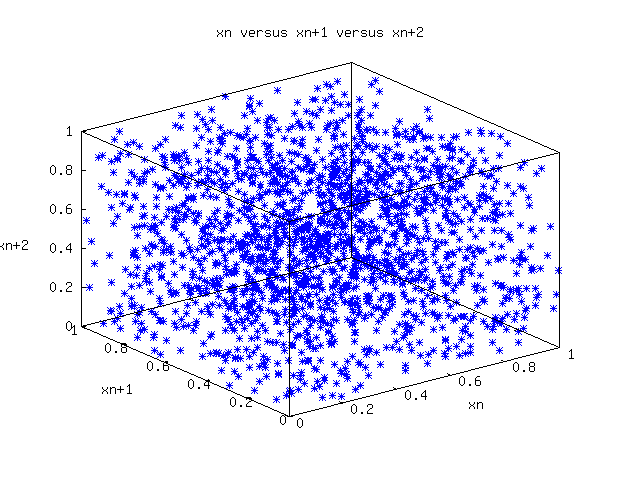
\includegraphics[width=8cm]{ecuyer3D_1}
\caption{Gr\'afica de $x_{n}$ versus $x_{n+1}$ versus $x_{n+2}$}
\end{figure}

\begin{figure}[ht]
\label{fig:ecuyer_3D_2}
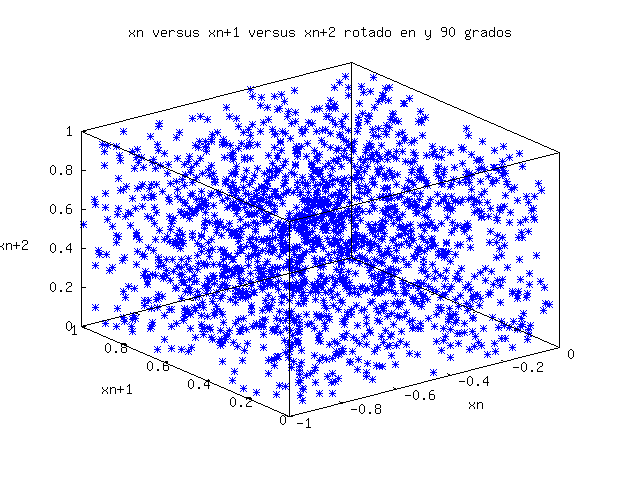
\includegraphics[width=8cm]{ecuyer3D_2}
\caption{Gr\'afica de $x_{n}$ versus $x_{n+1}$ versus $x_{n+2}$}
\end{figure}

\begin{figure}[ht]
\label{fig:ecuyer_3D_3}
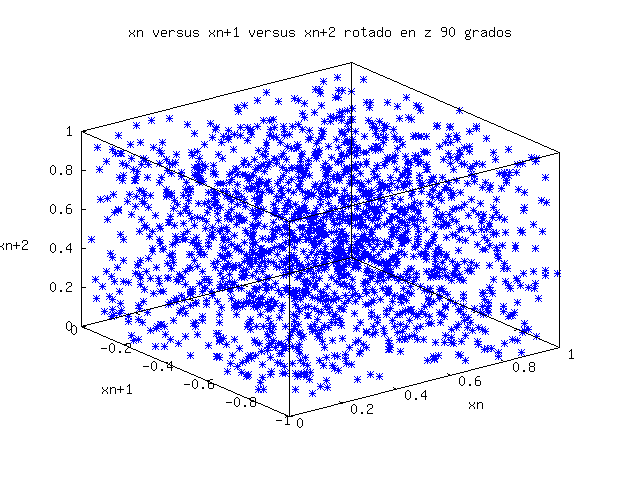
\includegraphics[width=8cm]{ecuyer3D_3}
\caption{Gr\'afica de $x_{n}$ versus $x_{n+1}$ versus $x_{n+2}$}
\end{figure}

Sin embargo, no se puede concluir que el generador de L'Ecuyer es un buen generador de n\'umeros
pseudoaleatorios. Sino, que ha pasado los tests Chi Cuadrado, Kolmogorov-Smirnov y que en sus
gr\'aficas no se presentan hiperplanos.

\section{Transformando a L'Ecuyer}
\label{sec:triangle}

A partir del generador de L'Ecuyer se desea obtener un generador de n\'umeros
pseudoaleatorios distribuidos seg\'un una funci\'on densidad triangular.\\
Para realizar \'esto se utiliza la t\'ecnica de la transformada inversa.

\begin{figure}[ht]
\begin{theorem}
\label{theo:1}
Sea $X$ una variable aleatoria con funci\'on de distribuci\'on $F(x)$
y se define:
$$U=F(X)$$
entonces $U$ es una variable aleatoria uniformemente distribuida en el intervalo $(0,1)$.
\end{theorem}
\end{figure}

Dicha t\'ecnica est\'a basada en el teorema \ref{theo:1} y consiste
en, dado un n\'umero $u$ que es una realizaci\'on de $U\sim\mathcal{U}[0,1]$,
entonces $x = F^{-1}(u)$ es una realizaci\'on de una VA $X$ con funci\'on
distribuci\'on $F(x)$.\\

La funci\'on de densidad triangular es \eqref{eq:triangle}. Su gr\'afica se observa
en la figura \ref{fig:triangle_fun}. A partir de ella podemos obtener
la funcio\'on distribuci\'on de probabilidad de $X$
\eqref{eq:triangleDistribution}.


\begin{figure}[ht]
\label{fig:triangle_fun}
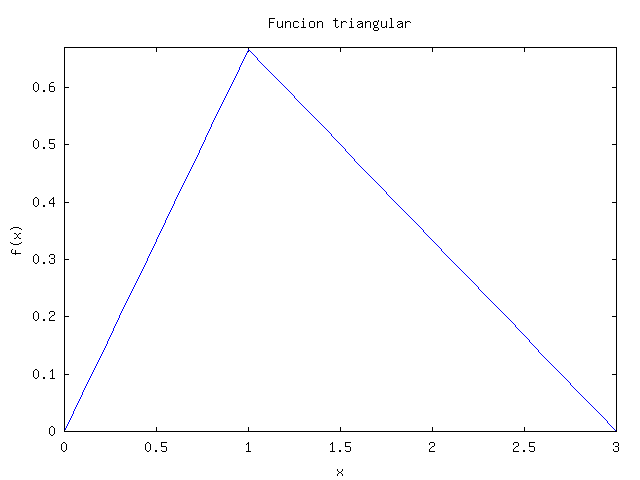
\includegraphics[width=8cm]{triangular}
\caption{Funci\'on de densidad triangular para $a=0$, $b=1$ y $c=3$}
\end{figure}


\begin{equation}
\label{eq:triangle}
f_{X}(x) =
\begin{cases}
\frac{2(x-a)}{(b-a)(c-a)} \quad & \text{si } a \leq x \leq b \\
\frac{2(c-x)}{(c-b)(c-a)} \quad & \text{si } b < x \leq c \\
0 \quad & \text{en otro caso}
\end{cases}
\end{equation}

\begin{equation}
\label{eq:triangleDistribution}
F_{X}(x) =
\begin{cases}
\frac{(x-a)^{2}}{(b-a)(c-a)} \quad & \text{si } a \leq x \leq b \\
\frac{b-a}{c-a} + \frac{(x-b)(2c-x+b)}{(c-a)(c-b)} \quad & \text{si } b < x \leq c \\
1 \quad & \text{en otro caso}
\end{cases}
\end{equation}

Dada dicha funci\'on hallamos su inversa \eqref{eq:inverse}.\\

\begin{equation}
\label{eq:inverse}
F^{-1}_{X}(u) =
\begin{cases}
\sqrt{u(b-a)(c-a)}+a \quad & \\
\text{si } 0 \leq u \leq \frac{b-a}{c-a} & \\
-\sqrt{-u(c-a)(c-b)+(b-a)(c-b)+(c-b)^{2}} + c \quad & \\
\text{si } \frac{b-a}{c-a} < u \leq \frac{c-b}{c-a}+\frac{b-a}{c-a} \\
\end{cases}
\end{equation}

Luego, el algoritmo consiste en generar un n\'umero pseudoaleatorio $u$ utilizando
un generador de n\'umeros pseudaleatorios con distribuci\'on uniforme en el $[0,1]$ (como el generador de L'Ecuyer).
Finalmente, con $u$ se obtiene $F^{-1}_{X}(u)$ que es una realizaci\'on de la variable aleatoria $X$.
Los resultados obtenidos se pueden observar en la figura \ref{fig:triangle}.

\begin{figure}[ht]
\label{fig:triangle}
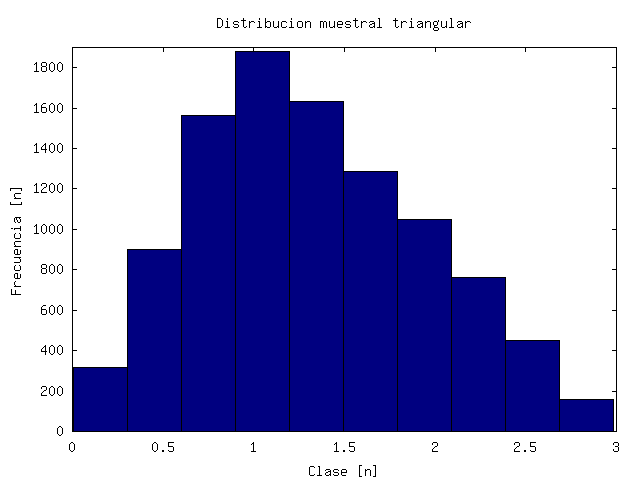
\includegraphics[width=8cm]{histograma_triangular}
\caption{Histograma de los n\'umeros obtenidos agrupados en 10 intervalos de clase}
\end{figure}

\section{Al infinito y m\'as all\'a}
\label{sec:buzzlightyear}

El sistema de propulsi\'on WARP de la nave espacial USS Enterprise,
deriva a dos propulsores en las nescellas laterales, ubicadas a
estribor y babor. Ambos propulsores son alimentados mediante un
N\'ucleo WARP en el interior de un reactor donde se llevan a
cabo reacciones de aniquilaci\'on materia-antimateria, moderadas
por cristales de dilitio. Los cristales de dilitio se procesan en
una c\'amara controlada, llamada Matriz de Dilitio.
Dicho subsistema posee una redundacia. La nave puede propulsarse
a velocidad WARP con una sola nescella operativa.

Los tiempos de operaci\'on de cada componente del sistema se muestran
en el cuadro \ref{tab:components}.

\begin{table}
\label{tab:components}
\centering
\begin{tabular}{|c|c|}
\hline
  C\'amara de Dilitio & $X_{1}\sim$Uniforme [20,50] horas \\
\hline
  C\'amara Redundante & $X_{2}\sim$Uniforme [5,12] horas \\
\hline
  Propulsor Babor & $X_{3}\sim$Exponencial $T_{3}=240$ horas \\
\hline
  Propulsor Estribor & $X_{4}\sim$Exponencial $T_{4}=240$ horas \\
\hline
  N\'ucleo WARP & $X_{5}\sim$Lineal creciente [12,72] horas \\
\hline
\end{tabular}
\end{table}

Si $x_i$ es una realizaci\'on de la variable $X_i$, entonces su funci\'on de distribuci\'on $f_{x1}$
se presenta en las ecuaciones \eqref{eq:dist_1}, \eqref{eq:dist_2},
\eqref{eq:dist_3y4}(tanto para $x_3$ como $x_4$) y \eqref{eq:dist_5}.

\begin{equation}
\label{eq:dist_1}
f_{X_1}(x) =
\begin{cases}
\frac{1}{30} & x \in [20,50] \\
0 & x \notin [20, 50]
\end{cases}
\end{equation}
\begin{equation}
\label{eq:dist_2}
f_{X_2}(x) =
\begin{cases}
\frac{1}{7} & x \in [5,12] \\
0 & x \notin [5,12]
\end{cases}
\end{equation}
\begin{equation}
\label{eq:dist_3y4}
f_{X_3, X_4}(x) =
  \begin{cases}
    \frac{1}{240} e^{-\frac{t}{240}} & t > 0 \\
    0 & t < 0
  \end{cases}
\end{equation}
\begin{equation}
\label{eq:dist_5}
f_{X_5}(x) =
\begin{cases}
\frac{x}{1800} - \frac{1}{150} & x \in [12,72] \\
0 & x \notin [12,72]
\end{cases}
\end{equation}

Luego, el tiempo de operaci\'on del sistema como un todo es una variable
aleatoria $T$ definida en base a las $X_i$ como se muestra en \eqref{eq:time}.
\begin{equation}
\label{eq:time}
T = \mathrm{min} \{ \mathrm{max} \{ X_1 , X_2 \}, X_5 , \mathrm{max} \{ X_3 , X_4 \} \}
\end{equation}

Por ende, el tiempo medio entre fallos del sistema se observa en \eqref{eq:integral_X},
con $i=1,2,3,4,5$.

\begin{eqnarray}
\label{eq:integral_X}
\mathcal{E} \{ T \} = \int\int\int\int\int\int_D \mathrm{min} 
\{ \mathrm{max} \{ x_1 , x_2 \}, x_5, \mathrm{max} \{ x_3 , x_4 \} \}
\nonumber
\\
f_{X_1}(x_1) f_{X_2}(x_2) f_{X_3}(x_3) f_{X_4}(x_4) f_{X_5}(x_5) d^5{x}
\end{eqnarray}

siendo $\mathcal{D}$ $[20;50]$ x $[5;12]$ x $[0,\infty]$ x $[0,\infty]$ x $[12;72]$. \\

Para poder estudiar el sistema mediante Montecarlo, debemos realizar el cambio
de variable que se muestra en \eqref{eq:trans_1}, \eqref{eq:trans_2},
\eqref{eq:trans_3}, \eqref{eq:trans_4}, \eqref{eq:trans_5}

\begin{eqnarray}
	\label{eq:trans_1}
	x_1 = 30 u_1 + 20 \\
	\label{eq:trans_2}
	x_2 = 7 u_2 + 5 \\
	\label{eq:trans_3}
	x_3 = - 240 \ln (1 - u_3) \\
	\label{eq:trans_4}
	x_3 = - 240 \ln (1 - u_4) \\
	\label{eq:trans_5}
	x_3 = 60 u_5 + 12 \\
\end{eqnarray}

siendo $u_i$ realizaciones de variables aleatorias $\mathcal{U}[0,1]$.
El determinante jacobiano de la transformaci\'on $J$ se observa en \eqref{eq:jacob}

\begin{equation}
\label{eq:jacob}
J =
\begin{vmatrix}
  30 & 0 & 0 & 0 & 0 \\
  0 & 7 & 0 & 0 & 0 \\
  0 & 0 & \frac{240}{1 - u_3} & 0 & 0 \\
  0 & 0 & 0 & \frac{240}{1 - u_4} & 0 \\
  0 & 0 & 0 & 0 & 60 \\
\end{vmatrix}
=
\frac {72576000}{(1 - u_3)(1 - u_4)}
\end{equation}

Finalmente, se reemplaza en \eqref{eq:integral_X} utilizando los cambios
de variable y el jacobiano computado. Se obtiene una nueva expresi\'on
del tiempo medio entre fallos del sistema \eqref{eq:integral_U}

\begin{eqnarray}
\label{eq:integral_U}
\mathcal{E} \{ T \} =	\int\limits_{[0,1]^6} \mathrm{min} 
\{ \mathrm{max}\{ 30 u_1 + 20, 7 u_2 + 5\} , 60 u_5 + 12,
\nonumber
\\
\mathrm{max}\{ -240 \ln ( 1 - u_3 ) , -240 \ln ( 1 - u_4 ) \} \} d^6u
\end{eqnarray}

Para realizar la simulaci\'on se utiliza el generador de n\'umeros
pseudo-aleatorios estudiado en la secci\'on \ref{sec:goingdown}. Se calculan
cinco secuencias, una para cada $u_i \in [0,1]$.

Para realizar la simulaci\'on se aplica Montecarlo. Como se realizan varias
simulaciones, las semillas de L'Ecuyer deben ir variando para obtener diversos
resultados. Dichas semillas son provistas por la funci\'on \textit{rand} del
aplicativo \textit{GNU-Octave} tomando como semilla el valor 0. \\
Se realizan $56$ realizaciones de la integral \eqref{eq:integral_U} que pueden
observarse en la figura \ref{fig:montecarlo}. De dichas realizaciones resulta
el estimador de tiempo medio de vuelo $\langle T \rangle = 29.874$ horas con
un desv\'io muestral $S = 9.2745$ horas. \\
Luego, para un nivel de significaci\'on del $5\%$ se aplica
\eqref{eq:student} para obtener el tiempo medio de vuelo. El mismo
resulta $ 29.874 \pm 0.7429 $ horas.\\
Cabe destacar el porqu\'e de la cantidad de simulaciones elegidas. Esto
se debe a que en cada iteraci\'on se realiza el c\'omputo
\eqref{eq:student_i} siendo $I_i$ el intervalo dado por \eqref{eq:student}
tomando  $t_{n-1,1-\alpha/2}=1.6$.
Luego, se pide que dicho c\'omputo tenga un error relativo menor al $5\%$,
obteniendo $56$ como n\'umero total de simulaciones.

\begin{equation}
\label{eq:student}
\langle T \rangle - t_{n-1,1-\alpha/2}\frac{S}{\sqrt{n}}
< \langle T \rangle <
\langle T \rangle + t_{n-1,1-\alpha/2}\frac{S}{\sqrt{n}}
\end{equation}

\begin{equation}
\label{eq:student_i}
\frac{I_i}{\langle T_i \rangle}
\end{equation}


\begin{figure}[ht]
\label{fig:montecarlo}
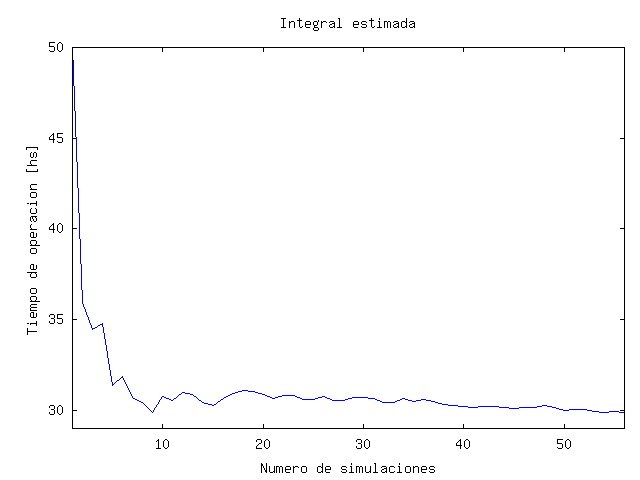
\includegraphics[width=8cm]{mean}
\caption{Realizaciones de la integral \ref{eq:integral_U} mediante Montecarlo}
\end{figure}

\begin{figure}[ht]
\label{fig:desvio}
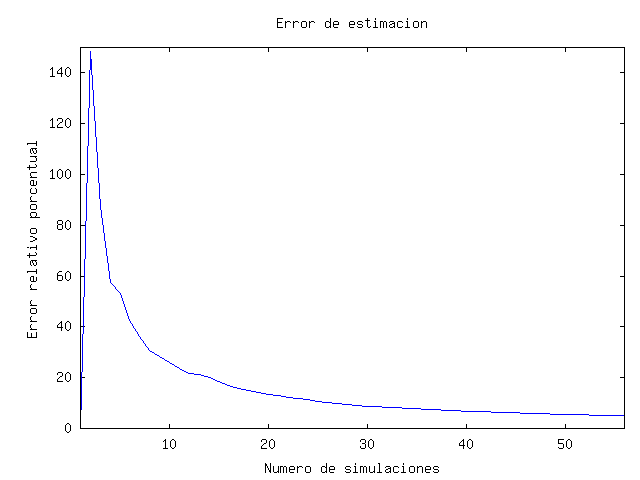
\includegraphics[width=8cm]{desv}
\caption{Error de estimaci\'on en funci\'on de la cantidad de simulaciones}
\end{figure}


\newpage

\section{Resultados Conclusiones}
\label{sec:conclusiones}
Los generadores de n\'umeros pseudaleatorios son necesarios para
realizar simulaciones de \'indole cient\'ifica como se observa
en el c\'omputo del timepo de vuelo del USS Enterprise.

\begin{thebibliography}{10}
\bibitem{chiTable} Tabla $\chi^{2}$.
\begin{verbatim}
http://www.wiphala.net/research/manual/
statistic/chi_cuadrado.html
\end{verbatim}
\bibitem{KSTable} Tabla Kolmogorov-Smirnov.
\begin{verbatim}
http://www.eridlc.com/onlinetextbook/
appendix/table7.htm
\end{verbatim} 
\bibitem{TStudentTable} Tabla T Student. \begin{verbatim}www.elosiodelosantos.com/sergiman/archivos/tablat.xls\end{verbatim}
\end{thebibliography}
\end{document}